
\subsection{THD} 
A continuación se muestra una tabla con los resultados del análisis de Fourier realizados con el \textbf{LTSpice} con el comando \textbf{SPICE} \textit{\textbf{.four}} para entrada de $1.0795 \si[per-mode=symbol]{\volt}$ pico (máxima excursión, $60 \si[per-mode=symbol]{\watt}$) a $1 \si[per-mode=symbol]{\kilo\hertz}$. 


%******************************************************************************************
\lstset{language=,xleftmargin=1em,numbers=none}

\lstset{showspaces=false}
\lstset{showstringspaces=false}
\normalfont
\normalsize
\lstset{backgroundcolor=\color{white},rulecolor=\color{blue}}
\lstset{basicstyle=\ttfamily\color{red}}

\lstset{keywordstyle=[1]\ttfamily\color{red}\bfseries}
\lstset{keywordstyle=[2]\ttfamily\color{red}}
\lstset{keywordstyle=[3]\ttfamily\bfseries\color{red}}
\lstset{keywordstyle=[4]\ttfamily\bfseries\color{red}}

\lstset{identifierstyle=\ttfamily\color{red}}
\lstset{commentstyle=\ttfamily\color{red}\textit}
\lstset{stringstyle=\ttfamily\color{red}\upshape}
\lstset{tabsize=4}

\lstset{numberstyle=\ttfamily\color{red}\upshape}
\lstset{numbersep=5pt}

\lstset{extendedchars=\false, inputencoding=utf8x}



\fontencoding{T1}
\fontseries{m}
\fontsize{7pt}{8pt}
\selectfont
%******************************************************************************************

\begin{lstlisting}
N-Period=4
Fourier components of V(out)
DC component:-0.00609365

Harmonic	Frequency	 Fourier 	Normalized	 Phase  	Normalized
 Number 	  [Hz]   	Component	 Component	[degree]	Phase [deg]
    1   	1.000e+03	3.099e+01	1.000e+00	   -0.07	    0.00
    2   	2.000e+03	4.065e-04	1.312e-05	   78.76	   78.83
    3   	3.000e+03	7.184e-04	2.318e-05	    6.71	    6.78
    4   	4.000e+03	1.003e-04	3.235e-06	   93.85	   93.93
    5   	5.000e+03	4.902e-05	1.582e-06	  170.68	  170.75
    6   	6.000e+03	4.829e-05	1.558e-06	  -59.26	  -59.18
    7   	7.000e+03	1.293e-04	4.172e-06	   26.87	   26.94
    8   	8.000e+03	1.457e-05	4.702e-07	  104.20	  104.28
    9   	9.000e+03	4.272e-05	1.379e-06	   52.46	   52.54
   10   	1.000e+04	3.185e-05	1.028e-06	  -70.05	  -69.98
   11   	1.100e+04	4.199e-05	1.355e-06	   67.89	   67.96
   12   	1.200e+04	1.060e-05	3.420e-07	  -93.43	  -93.35
   13   	1.300e+04	3.133e-05	1.011e-06	  136.68	  136.75
   14   	1.400e+04	6.583e-06	2.124e-07	  -84.68	  -84.61
   15   	1.500e+04	3.250e-05	1.049e-06	  153.79	  153.87
   16   	1.600e+04	5.378e-06	1.735e-07	  112.21	  112.28
   17   	1.700e+04	2.309e-05	7.450e-07	  156.75	  156.83
   18   	1.800e+04	9.952e-06	3.211e-07	  100.07	  100.15
   19   	1.900e+04	9.865e-06	3.183e-07	  104.44	  104.51
   20   	2.000e+04	9.097e-06	2.935e-07	   94.78	   94.86
   21   	2.100e+04	1.826e-05	5.892e-07	   40.20	   40.28
   22   	2.200e+04	4.168e-06	1.345e-07	   80.56	   80.64
   23   	2.300e+04	2.337e-05	7.541e-07	   31.93	   32.01
   24   	2.400e+04	2.081e-06	6.716e-08	  -37.14	  -37.07
   25   	2.500e+04	1.654e-05	5.337e-07	   33.14	   33.21
   26   	2.600e+04	4.155e-06	1.341e-07	  -67.28	  -67.21
   27   	2.700e+04	2.669e-06	8.613e-08	   61.95	   62.02
   28   	2.800e+04	2.670e-06	8.615e-08	  -78.19	  -78.12
   29   	2.900e+04	1.103e-05	3.558e-07	 -154.32	 -154.25
   30   	3.000e+04	1.358e-06	4.381e-08	  133.87	  133.94
Total Harmonic Distortion: 0.002742%(0.002742%)

\end{lstlisting}

\normalfont
\normalsize


La distorsión armónica simulada es de $0.0027 \si[per-mode=symbol]{\percent}$ en la máxima excursión a $1 \si[per-mode=symbol]{\kilo\hertz}$. El resultado para una simulación similar a $10 \si[per-mode=symbol]{\kilo\hertz}$ se muestra a continuación:



\clearpage



%******************************************************************************************
\fontencoding{T1}
\fontseries{m}
\fontsize{7pt}{8pt}
\selectfont
%******************************************************************************************


\begin{lstlisting}
N-Period=4
Fourier components of V(out)
DC component:-0.000245223

Harmonic	Frequency	 Fourier 	Normalized	 Phase  	Normalized
 Number 	  [Hz]   	Component	 Component	[degree]	Phase [deg]
    1   	1.000e+04	3.099e+01	1.000e+00	   -0.86	    0.00
    2   	2.000e+04	1.108e-03	3.575e-05	  -55.41	  -54.55
    3   	3.000e+04	8.353e-04	2.695e-05	   29.81	   30.67
    4   	4.000e+04	7.803e-04	2.518e-05	 -104.83	 -103.97
    5   	5.000e+04	1.439e-04	4.644e-06	 -166.50	 -165.64
    6   	6.000e+04	7.527e-04	2.429e-05	  -81.99	  -81.13
    7   	7.000e+04	3.855e-04	1.244e-05	   78.77	   79.62
    8   	8.000e+04	4.484e-04	1.447e-05	 -108.78	 -107.92
    9   	9.000e+04	9.610e-05	3.101e-06	  123.98	  124.84
   10   	1.000e+05	3.037e-04	9.801e-06	  -83.93	  -83.08
   11   	1.100e+05	8.219e-05	2.652e-06	   78.36	   79.22
   12   	1.200e+05	8.684e-05	2.802e-06	 -108.53	 -107.67
   13   	1.300e+05	1.085e-04	3.501e-06	  -84.14	  -83.29
   14   	1.400e+05	1.247e-05	4.025e-07	   51.25	   52.11
   15   	1.500e+05	1.942e-04	6.267e-06	  -76.55	  -75.70
   16   	1.600e+05	5.183e-05	1.672e-06	  120.09	  120.95
   17   	1.700e+05	2.269e-04	7.322e-06	  -81.74	  -80.89
   18   	1.800e+05	6.231e-05	2.011e-06	  175.95	  176.80
   19   	1.900e+05	1.662e-04	5.363e-06	  -93.66	  -92.81
   20   	2.000e+05	1.084e-04	3.497e-06	 -148.53	 -147.67
   21   	2.100e+05	8.073e-05	2.605e-06	 -146.75	 -145.89
   22   	2.200e+05	1.279e-04	4.126e-06	 -133.60	 -132.74
   23   	2.300e+05	1.299e-04	4.191e-06	  140.65	  141.51
   24   	2.400e+05	8.677e-05	2.800e-06	 -118.21	 -117.35
   25   	2.500e+05	1.712e-04	5.526e-06	  120.85	  121.70
   26   	2.600e+05	3.611e-05	1.165e-06	  -30.78	  -29.93
   27   	2.700e+05	1.205e-04	3.889e-06	  108.09	  108.95
   28   	2.800e+05	9.993e-05	3.225e-06	   27.09	   27.94
   29   	2.900e+05	1.951e-05	6.297e-07	   16.45	   17.31
   30   	3.000e+05	1.251e-04	4.037e-06	   39.61	   40.47
Total Harmonic Distortion: 0.006334%(0.010095%)

\end{lstlisting}

\normalfont
\normalsize


La distorsión total es de $0.006 \si[per-mode=symbol]{\percent}$. Haciendo simulaciones similares se obtiene que para $1 \si[per-mode=symbol]{\watt}$ ($4 \si[per-mode=symbol]{\volt}$) de salida, y $1 \si[per-mode=symbol]{\kilo\hertz}$, la distorsión es de $0.000217 \si[per-mode=symbol]{\percent}$ y a $10 \si[per-mode=symbol]{\kilo\hertz}$, $0.002 \si[per-mode=symbol]{\percent}$. En todos los casos se cumple lo especificado.




En la figura~\figref{fig:distorsion-barrido-1} se muestra la distorsión a $1 \si[per-mode=symbol]{\kilo\hertz}$ en función de la potencia de salida y en la figura~\figref{fig:distorsion-barrido-2} lo mismo, pero a $10 \si[per-mode=symbol]{\kilo\hertz}$.

\clearpage


\begin{figure}[H]
	\centering
	\includegraphics[width=0.7\paperheight, angle=90]{img/sims/distorsion-barrido-1.png}
	\caption{Distorsión a $1 \si[per-mode=symbol]{\kilo\hertz}$ a distintos valores de potencia de salida.}
	\label{fig:distorsion-barrido-1}
\end{figure}

\clearpage


\begin{figure}[H]
	\centering
	\includegraphics[width=0.7\paperheight, angle=90]{img/sims/distorsion-barrido-2.png}
	\caption{Distorsión a $10 \si[per-mode=symbol]{\kilo\hertz}$ a distintos valores de potencia de salida.}
	\label{fig:distorsion-barrido-2}
\end{figure}

\clearpage

\begin{figure}[H]
	\centering
	\includegraphics[width=0.7\paperheight, angle=90]{img/sims/distorsion-frec.png}
	\caption{Distorsión a máxima excursión en función de la frecuencia.}
	\label{fig:distorsion-frec}
\end{figure}

\clearpage



Los valores de distorsión bajan a potencias menores porque se reduce la distorsión por alinealidad de los transistores: mientras más chica es la excursión, más uno se encuentra en pequeña señal, y más lineal es la relación entre $v_{be}$ e $i_{c}$. Por otra parte, se colocó al multiplicador de $V_{be}$ de modo tal que haga funcionar a la etapa de salida en modo A-B, reduciendo la distorsión por crossover, de todos modos se puede observar como a partir de alrededor $12 \si[per-mode=symbol]{\watt}$, que corresponde a una tensión de alrededor de $14 \si[per-mode=symbol]{\volt}$, tensión a la cual se empieza a producir el sewitcheo de los transistores externos, la distorsión deja de crecer linealmente por pasar a estar dominada por la distorsión de switching en lugar de la de crossover.

La figura~\figref{fig:distorsion-frec}, por su parte, muestra resultados de simulaciones de distorsión a máxima excursión en función de la frecuencia, puede verse como alrededor de los $80 \si[per-mode=symbol]{\kilo\hertz}$ crece mas abruptamente la distorsión, esto se justifica en la próxima sección con el Slew-Rate del circuito, puede verse como la distorsión crece acercándose al $12 \si[per-mode=symbol]{\percent}$ que corresponde a una triangular.



\subsection{Slew Rate} Simulando una entrada escalón en el amplificador, se observa la salida de la figura~\figref{fig:slew_zoom} en la carga.

La pendiente es de $19.3 \si[per-mode=symbol]{\volt\per\micro\second}$. Esto es mayor a la máxima pendiente de la salida en máxima potencia a la máxima frecuencia especificada de $30 \si[per-mode=symbol]{\kilo\hertz}$, por lo que el ancho de banda de potencia cumplirá lo especificado ($15 \si[per-mode=symbol]{\volt\per\micro\second} < 19.3 \si[per-mode=symbol]{\volt\per\micro\second} $).

Para hallar el SR de manera teórica, partimos de la fuente de corriente de un par diferencial. La corriente que generan es de $3.15 \si[per-mode=symbol]{\milli\ampere}$, es decir, $1.57 \si[per-mode=symbol]{\milli\ampere}$ por rama. Si dividimos este valor por el capacitor de Miller ($100 \si[per-mode=symbol]{\pico\farad}$), nos queda un SR de $15.7 \si[per-mode=symbol]{\volt\per\micro\second}$. Si calculamos el ancho de banda de potencia, con este \textbf{SR}, nos da que la frecuencia máxima a la que el amplificador puede desarrollar $31 \si[per-mode=symbol]{\volt}$ pico, de salida, es $80.6 \si[per-mode=symbol]{\kilo\hertz}$. A pesar de que el \textbf{SR} nos dio menos que en la simulación, el ancho de banda sigue cumpliendo con las especificaciones. Esta diferencia se debe a que la simulación utiliza un método numérico para hallar las respuestas con un error pequeño, y el cálculo teórico se basa en varias hipótesis para simplificar el cálculo. Será importante, a la hora de armar el circuito, que éste funcione dentro de los parámetros esperados.

\clearpage

\begin{figure}[H]
	\centering
	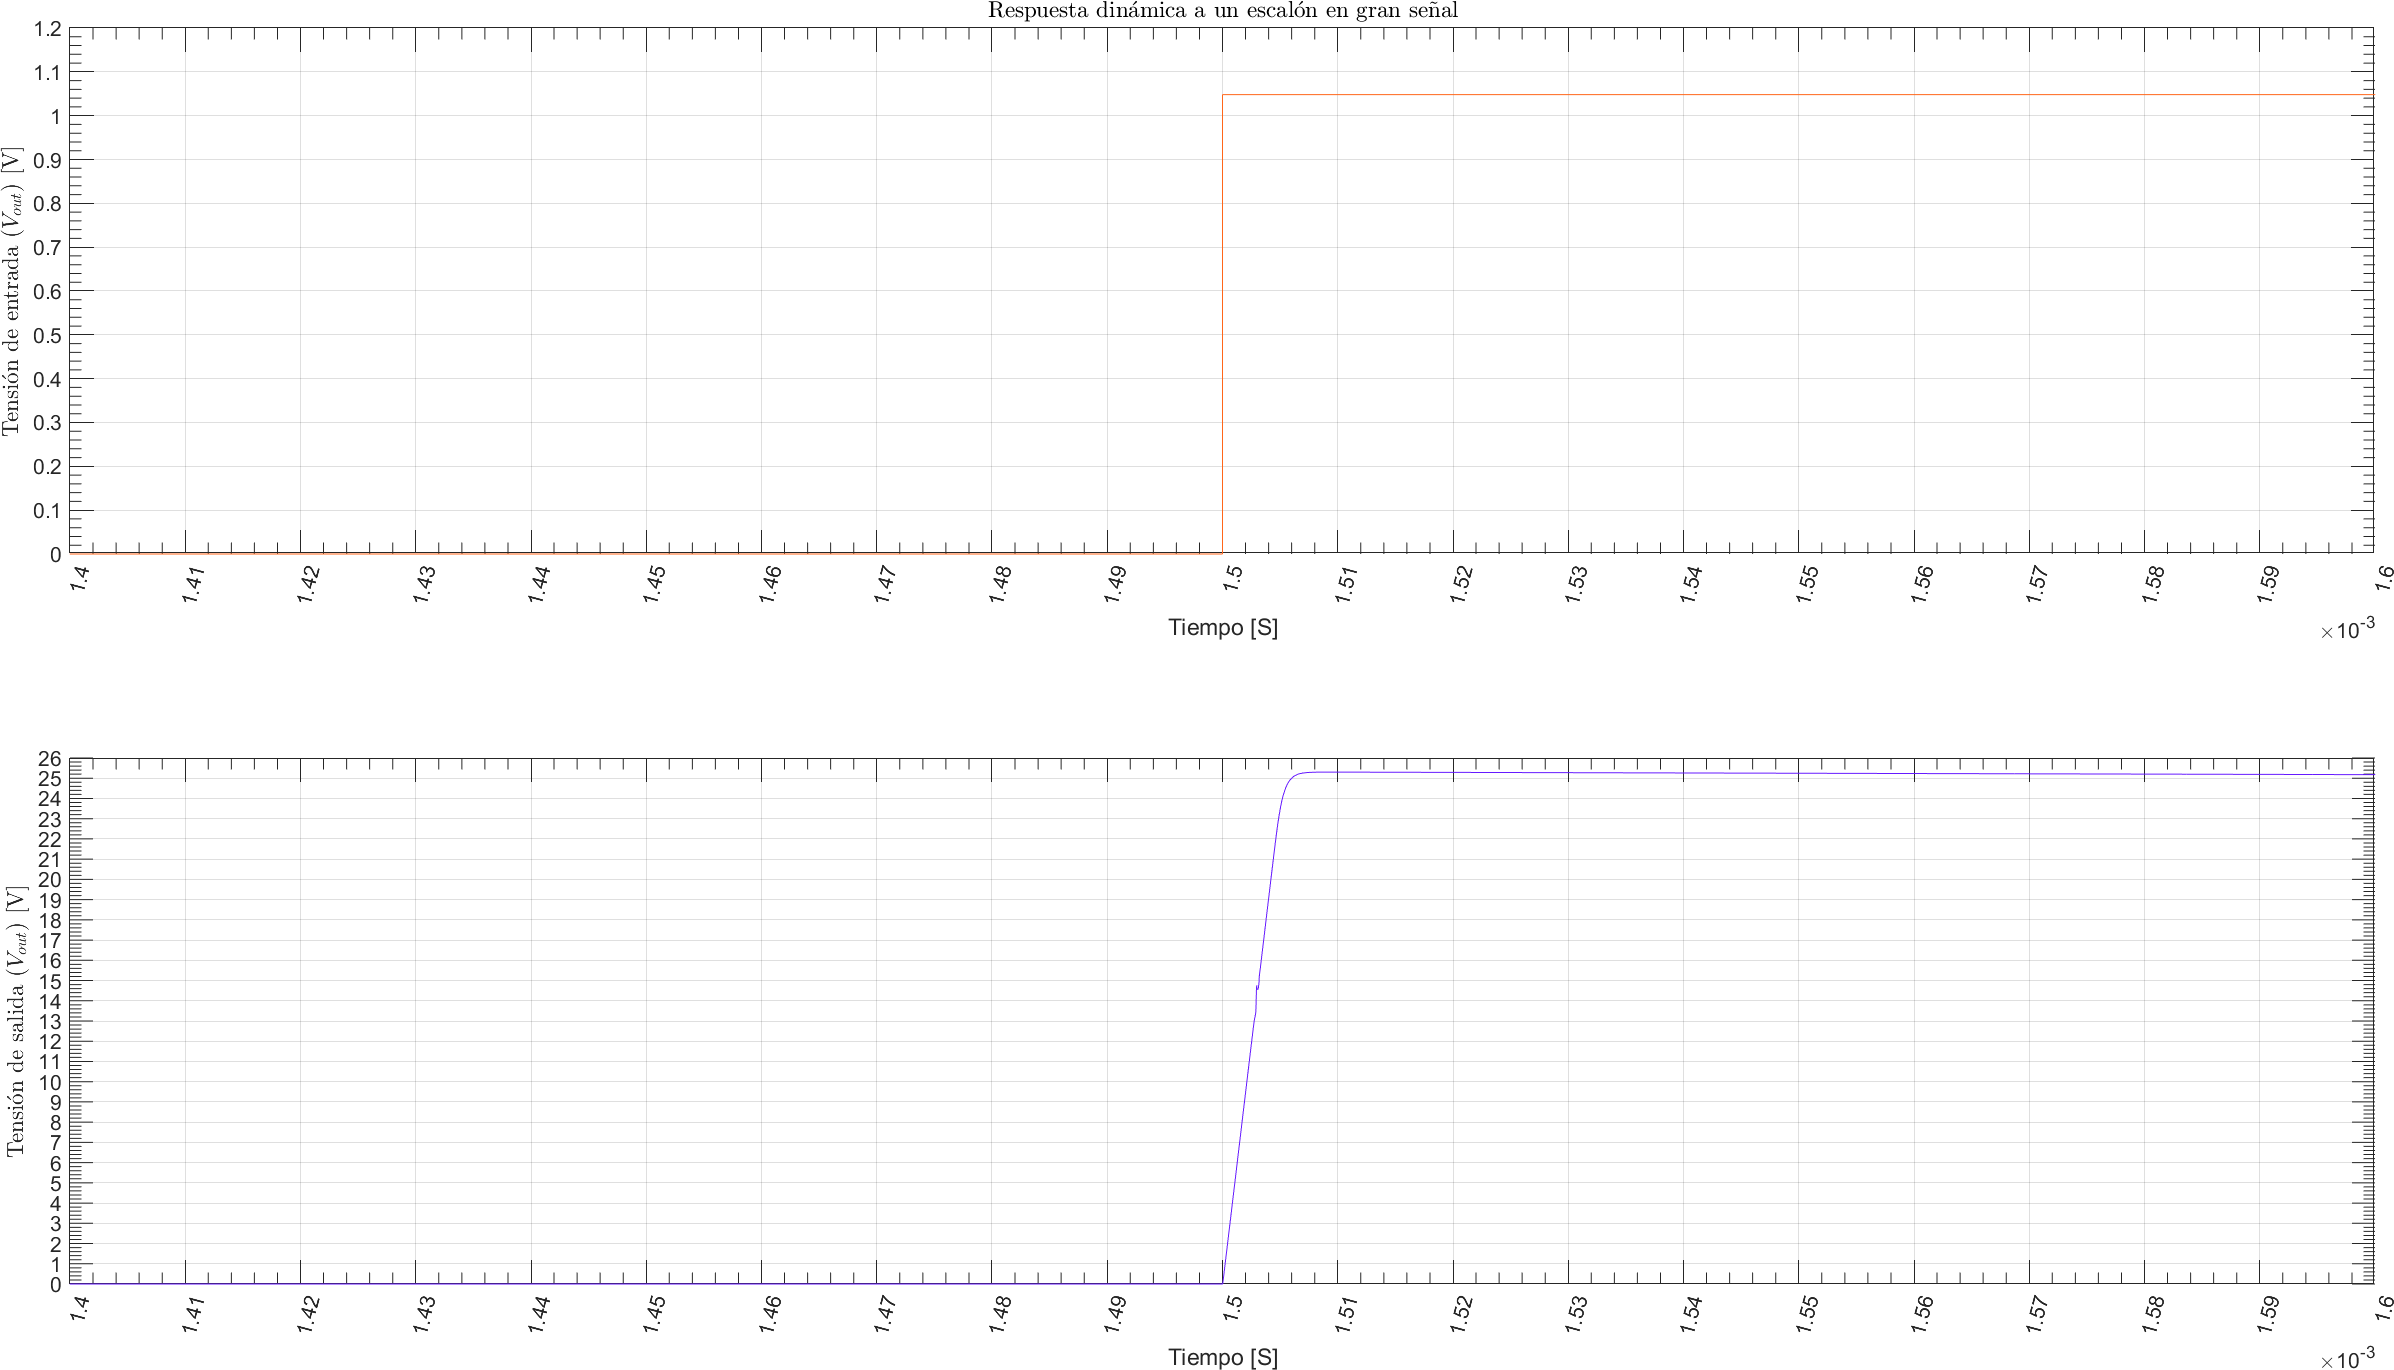
\includegraphics[width=0.7\paperheight, angle=90]{img/sims/Slew_Rate.png}
	\caption{Respuesta frente a una entrada escalón.}
	\label{fig:slew}
\end{figure}

\clearpage

\begin{figure}[H]
	\centering
	\includegraphics[width=0.7\paperheight, angle=90]{img/sims/Slew_Rate_Zoom.png}
	\caption{Respuesta frente a una entrada escalón, zoom sobre la pendiente.}
	\label{fig:slew_zoom}
\end{figure}

\clearpage

\subsection{CMRR - factor de rechazo de modo común}

Un amplificador diferencial ideal debería amplificar, como dice su nombre, las diferencias entre las tensiones de entrada, e ignorar la tensión media. El parámetro \textbf{CMRR} mide cuan bien esto se logra, como el cociente entre la ganancia de modo común $A_{c}$ y la de modo diferencial $A_{d}$. 

\subsubsection{Modo común} 

Se simuló la primera etapa frente una entrada común de $100 \si[per-mode=symbol]{\milli\volt}$ con el circuito de la figura~\figref{fig:ac} y se obtuvo la ganancia de modo común. Para cada par diferencial del doble par, cuyas salidas son $o_{1}$ y $o_{2}$ en la figura~\figref{fig:ac}, se obtuvieron $A_{d}^{NPN}=\frac{V_{o_{1}}}{100 \si[per-mode=symbol]{\milli\volt}}$ y $A_{d}^{PNP}=\frac{V_{o_{2}}}{100 \si[per-mode=symbol]{\milli\volt}}$ como la relación entre la salida (pico) correspondiente al par y la entrada común (pico). 


\begin{figure}[H]
	\centering
	\includegraphics[height=0.2\textwidth]{img/sims/ac.png}
	\caption{Circuito usado para simular la amplificación de modo común.}
	\label{fig:ac}
\end{figure}

\subsubsection{Modo diferencial}

La amplificación de modo diferencial se obtuvo de forma análoga, con las fuentes de la figura~\figref{fig:ac} conectadas a contrafase. Las tensiones pico de las fuentes usadas fueron de sólo $1 \si[per-mode=symbol]{\milli\volt}$ porque se esperaba una amplificación mucho mayor que para el caso de modo común. Es decir, $A_{d}^{NPN}=\frac{V_{o_{1}}}{2 \si[per-mode=symbol]{\milli\volt}}$, y $A_{d}^{PNP}=\frac{V_{o_{2}}}{2 \si[per-mode=symbol]{\milli\volt}}$.

\subsubsection{CMRR} 

El factor de rechazo es simplemente $\frac{A_{d}}{A_{c}}$, en valor absoluto.


\begin{table}[H]
\centering
\begin{tabular}{l|ll}
 & NPN & PNP \\ \hline
$A_{c}$ & $-36.23 \si[per-mode=symbol]{\decibel}$ & $-41.32 \si[per-mode=symbol]{\decibel}$  \\
$A_{d}$ & $35.37 \si[per-mode=symbol]{\decibel}$ & $36.49 \si[per-mode=symbol]{\decibel}$  \\
RRMC & $71.6 \si[per-mode=symbol]{\decibel}$ & $77.81 \si[per-mode=symbol]{\decibel}$  
\end{tabular}
\end{table}

\clearpage

\subsection{\textbf{PSRR} - factor de rechazo del ripple la fuente}

El \textbf{PSRR} se define como la relación entre el cambio en la tensión de alimentación y el cambio equivalente en la tensión de entrada. Idealmente este valor sería infinito.

Simulando utilizando una fuente en forma de rampa invertida de $100 \si[per-mode=symbol]{\hertz}$ en serie con las fuentes de alimentación, pasivando la fuente de entrada y midiendo la amplitud de la señal de $100 \si[per-mode=symbol]{\hertz}$ y sus armónicos resultantes a la salida se obtuvo:

\[ PSRR := {\Delta V_\mathrm{fuente} \over {\Delta V_\mathrm{o}}} \cdot A_d = 111.3 \si[per-mode=symbol]{\decibel} \]



Es decir, con la ganancia de $29 \si[per-mode=symbol]{\decibel}$ de este circuito, por cada $1 \si[per-mode=symbol]{\volt}$ de ripple en la fuente de $+49 \si[per-mode=symbol]{\volt}$ se superponen aproximadamente $76.74 \si[per-mode=symbol]{\micro\volt}$ en la salida ($111.3 \si[per-mode=symbol]{\decibel} - 29 \si[per-mode=symbol]{\decibel} = 82.3 \si[per-mode=symbol]{\decibel}$ y $10^\frac{-82.3}{20} \cong 76.74 \si[per-mode=symbol]{\micro\volt} $)

También, se simuló y verificó el comportamiento correcto del amplificador para una posible caída de tensión en los rieles del $20 \si[per-mode=symbol]{\percent}$: sólo se reduce la máxima excursión, de donde se tomó la máxima excursión de $31 \si[per-mode=symbol]{\volt}$ en esta, la peor condición.

En nuestro caso, al utilizarse una fuente de alimentación no regulada, es realmente importante el rechazo de ripple de la fuente, ya que este es del orden de $2.5 \si[per-mode=symbol]{\volt}$ de pico cuando el amplificador está funcionando a máxima potencia, según lo simulado.

\subsection{Resistencia de salida}  

Para la simulación de la resistencia de salida, se colocó una fuente de corriente alterna de $1 \si[per-mode=symbol]{\ampere}$ a la salida, con la entrada pasivada, y se capturó la tensión de salida en un barrido de frecuencias.


El circuito simulado, con una caja representando el amplificador, se observa en la figura~\figref{fig:circuito_r-out-current}.


\begin{figure}[H]
	\centering
	\includegraphics[width=0.6\textwidth]{img/sims/circuito-r_out-current.png}
	\caption{Circuito usado para simular la resistencia de salida. La caja representa al amplificador.}
	\label{fig:circuito_r-out-current}
\end{figure}

Los resultados del barrido se muestran en la figura~\figref{fig:R_out}, y un zoom en las frecuencias de trabajo especificadas en la figura~\figref{fig:R_out-zoom}.

\begin{figure}[H]
	\centering
	\includegraphics[width=0.8\textwidth]{img/sims/R_out.png}
	\caption{Barrido en frecuencias de la impedancia de salida simulada.}
	\label{fig:R_out}
\end{figure}

\begin{figure}[H]
	\centering
	\includegraphics[width=0.8\textwidth]{img/sims/R_out-zoom.png}
	\caption{Barrido en frecuencias de la impedancia de salida simulada para frecuencias hasta $30 \si[per-mode=symbol]{\kilo\hertz}$.}
	\label{fig:R_out-zoom}
\end{figure}

El módulo de la media geométrica de la impedancia de salida para las frecuencias entre $1 \si[per-mode=symbol]{\hertz}-30 \si[per-mode=symbol]{\kilo\hertz}$ es $11 \si[per-mode=symbol]{\milli\ohm}$.

\[ R_{out}\cong 11 \si[per-mode=symbol]{\milli\ohm}\]

La realimentación global serie-paralelo logra que la resistencia de salida sea muy baja, tanto que las resistencias parásitas pueden terminar siendo un factor no despreciable. Si se desprecian, el factor de amortiguamiento es  $DP \cong 730$, cumpliendo cómodamente con lo especificado.



\subsection{Resistencia de entrada}

Se simuló en el cociente entre la tensión de entrada y la corriente entregadas por el generador, para un barrido de frecuencias. El módulo de la media geométrica de la impedancia para las frecuencias entre $1 \si[per-mode=symbol]{\hertz}-30 \si[per-mode=symbol]{\kilo\hertz}$ es $35.28 \si[per-mode=symbol]{\kilo\ohm}$.

\[ R_{in}=35.28 \si[per-mode=symbol]{\kilo\ohm} \]

En la figura~\figref{fig:R_i} se puede ver un barrido en frecuencias de la resistencia de entrada para pequeña señal.


\begin{figure}[H]
	\centering
	\includegraphics[width=0.8\textwidth]{img/sims/R_i.png}
	\caption{Resistencia de entrada. Cociente entre tensión y corriente de entrada simuladas para pequeña señal de distintas frecuencias.}
	\label{fig:R_i}
\end{figure}



\subsection{Ancho de banda de potencia}


En la figura~\figref{fig:power_BW} se puede observar el gráfico de módulo y fase del ancho de banda de potencia para el amplificador, el ancho de banda obtenido es de $798.45 \si[per-mode=symbol]{\kilo\hertz}$, pero como sabemos mucho antes que esta frecuencia, a $80.6 \si[per-mode=symbol]{\kilo\hertz}$, el Slew-Rate limitará la excursión del amplificador, no obstante se cumple holgadamente con la especificación establecida de  $30 \si[per-mode=symbol]{\kilo\hertz}$ de ancho de banda de potencia, aún teniendo en cuenta la limitación por Slew-Rate.


\clearpage

\begin{figure}[H]
	\centering
	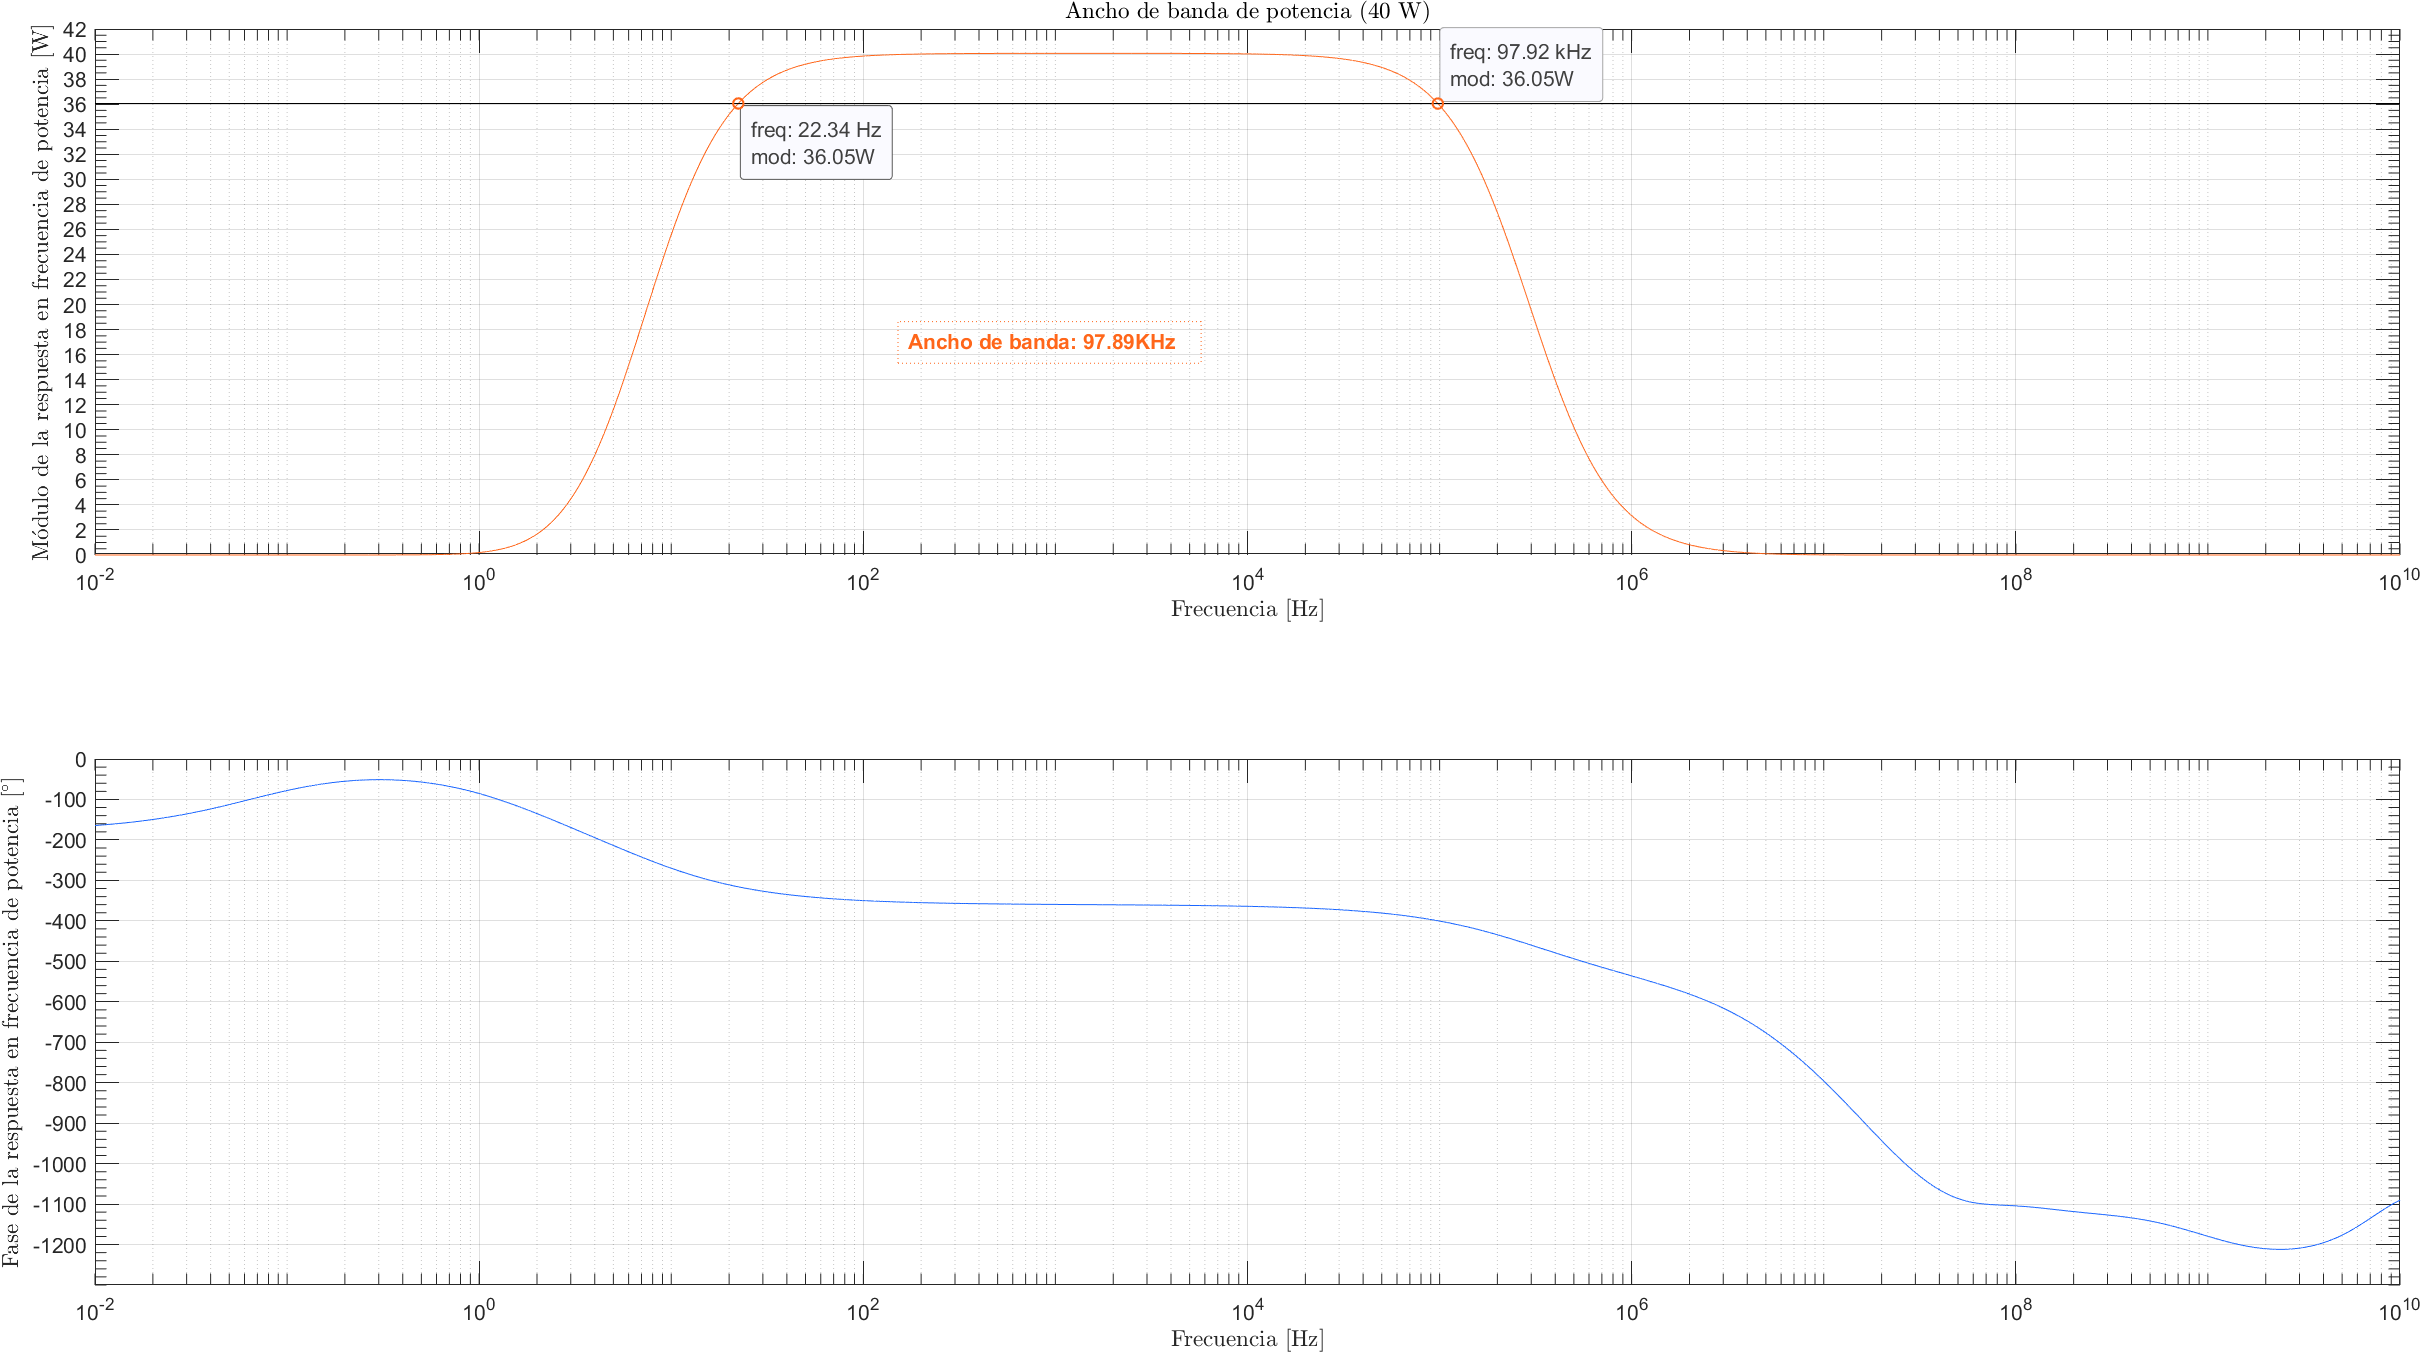
\includegraphics[width=0.7\paperheight, angle=90]{img/sims/Power_BW.png}
	\caption{Ancho de banda de potencia.}
	\label{fig:power_BW}
\end{figure}

\clearpage




